%%% Template originaly created by Karol Kozioł (mail@karol-koziol.net) and modified for ShareLaTeX use

\documentclass[a4paper,11pt]{article}

\usepackage[T1]{fontenc}
\usepackage[utf8]{inputenc}
\usepackage{graphicx,wrapfig}
\usepackage{xcolor}
\usepackage{parskip}
\usepackage{tgtermes}

\usepackage[
pdftitle={Math Assignment}, 
pdfauthor={Lucas Varela},
colorlinks=true,linkcolor=blue,urlcolor=blue,citecolor=blue,bookmarks=true,
bookmarksopenlevel=2]{hyperref}
\usepackage{amsmath,amssymb,amsthm,textcomp}
\usepackage{enumerate}
\usepackage{multicol}
\usepackage{tikz}
\usepackage{float}
\usepackage{caption}
\usepackage{geometry}
\geometry{total={210mm,297mm},
left=25mm,right=25mm,%
bindingoffset=0mm, top=20mm,bottom=20mm}


\linespread{1.0}

\newcommand{\linia}{\rule{\linewidth}{0.5pt}}


% my own titles
\makeatletter
\renewcommand{\maketitle}{
\begin{center}
\vspace{2ex}
{\huge \textsc{\@title}}
\vspace{1ex}
\\
\linia\\
\@author \hfill \@date
\vspace{4ex}
\end{center}
}
\makeatother
%%%

% custom footers and headers
\usepackage{fancyhdr,lastpage}
\pagestyle{fancy}
\lhead{}
\chead{}
\rhead{}
\lfoot{}
\cfoot{}
\rfoot{Page \thepage\ /\ \pageref*{LastPage}}
\renewcommand{\headrulewidth}{0pt}
\renewcommand{\footrulewidth}{0pt}
%

%%%----------%%%----------%%%----------%%%----------%%%

\begin{document}

\title{ Centro de Masa \& Momento de Inercia}

\author{Física I}

\date{\today}

\maketitle
\tableofcontents
\setlength\intextsep{-15pt}


\section{Centro de Masa}

\textbf{Partículas puntuales:}


\begin{wrapfigure}{r}{6.0cm}
	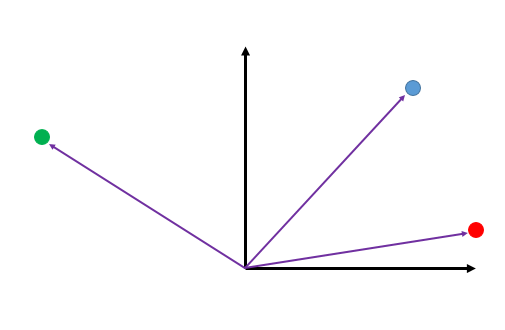
\includegraphics[scale=0.5]{./im/masaspuntuales}
\end{wrapfigure}
El centro de masa para un sistema discreto de $N$ partículas puntuales  está dado por:

\begin{equation}
 \vec{r}_{cm}  = \frac{m_1\vec{r}_1 + \dots + m_N \vec{r}_N}{m_1 + \dots + m_N}
\end{equation}

Donde $ \vec{r}_k$ es la posición de la k-ésima partícula y $m_k$ su masa.

\textbf{Distribución continua:}


\begin{wrapfigure}{r}{6.0cm}
	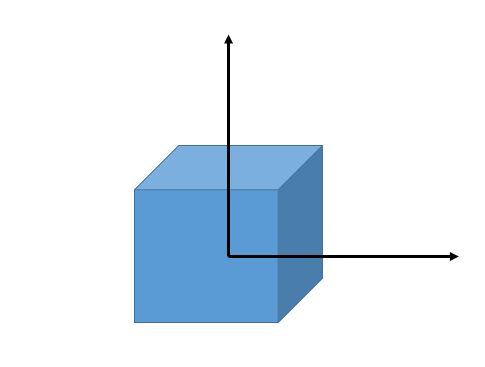
\includegraphics[scale=0.5]{./im/3d}
\end{wrapfigure}


El centro de masa de un objeto con distribución de masa continua viene dado por la siguiente integral:

\begin{equation}
 \vec{r}_{cm} = \frac{1}{M} \int \vec{r} dm
\end{equation}

Donde $M$ es la masa total del objeto. Existen tres casos a considerar: objetos de 1, 2 y 3 dimensiones. Para cada una respectivamente existe una densidad asociada:

\begin{subequations}
	\begin{align}
	\lambda &= \frac{d m}{dx} \\
	\sigma &= \frac{d m}{dA} \\
	\rho &= \frac{d m}{dV} 
	\end{align}
\end{subequations}

Donde $\lambda$ es la densidad lineal, $\sigma$ la densidad superficial y $\rho$ la densidad (se omite decir densidad volumétrica, se le dice solo densidad usualmente). Con ellas se puede obtener las siguientes expresiones para el centro de masa de distribuciones continuas:

\begin{subequations}
	\begin{align}
	\vec{r}_{cm} &= \frac{1}{M} \int \vec{r} \lambda \;dx  \\
	\vec{r}_{cm} &= \frac{1}{M} \int \int \vec{r} \sigma \;dA \\
	\vec{r}_{cm} &= \frac{1}{M} \int \int \int \vec{r} \rho\; dV 
	\end{align}
\end{subequations}


\textbf{Sistema de múltiples distribuciones continuas:}\\



\begin{wrapfigure}{r}{7.0cm}
	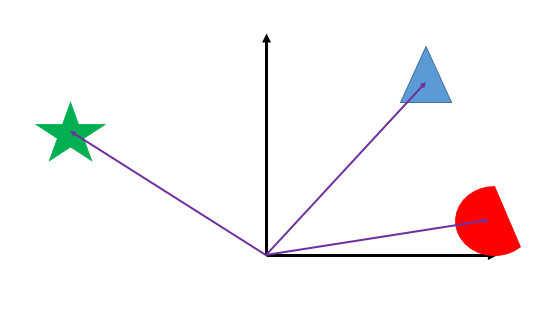
\includegraphics[scale=0.5]{./im/muchos3d}
\end{wrapfigure}

El centro de masa para un sistema de $N$ objetos de distribución continua está dado por:

\begin{equation}
 \vec{r}_{cm} = \frac{m_1\vec{r}_1 + \dots + m_N \vec{r}_N}{m_1 + \dots + m_N}
\end{equation}



Donde $ \vec{r}_k$ es el centro de masa del k-ésimo elemento y $m_k$ su masa.


\subsection{Ejemplo: Lamina de densidad uniforme} 


\begin{wrapfigure}{r}{7.0cm}
	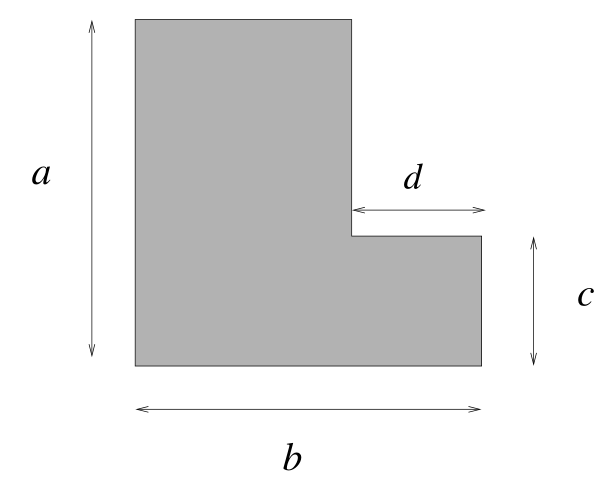
\includegraphics[scale=0.5]{./im/4}
\end{wrapfigure}

Se quiere encontrar la posición del centro de masa de la lamina mostrada en la figura. La masa total
de la lamina está repartida de manera uniforme en toda su superficie. \\

Para ello se utiliza la siguiente estrategia: se divide la figura en dos rectángulos y se encuentra el centro de masa para cada uno, luego aplicando la ecuación para calcular el centro de masa de múltiples distribuciones continuas se calcula el centro de masa de la figura entera:


\begin{wrapfigure}{r}{7.0cm}
	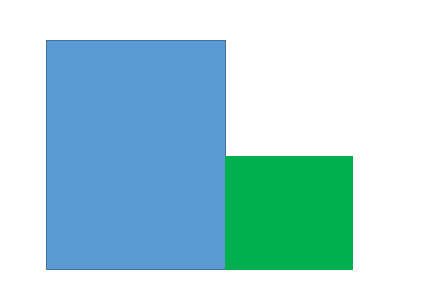
\includegraphics[scale=0.5]{./im/recdiv}
\end{wrapfigure}



\begin{wrapfigure}{r}{7.0cm}
	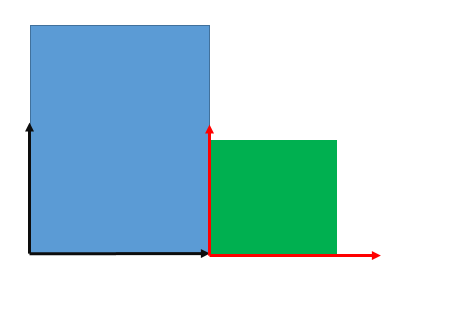
\includegraphics[scale=0.5]{./im/vert}
\end{wrapfigure}
Ahora, el centro de masa de cada rectángulo con respecto a ejes que estén en sus respectivos vértices inferiores izquierdos(ver figura) corresponde a la mitad de la altura y la mitad del ancho de cada uno.


Entonces el del rectángulo azul es:

$$ \vec{r}_a = \frac{b-d}{2} \hat{i} + \frac{a}{2} \vec{j}  $$

El del rectángulo verde con respecto a las coordenadas rojas es:

\color{red}

$$ \vec{r}_v = \frac{d}{2} \hat{i} + \frac{c}{2}\hat{j}$$

\color{black}
Ahora queremos saber estas posiciones con respecto al mismo sistema de coordenadas. Vemos que las coordenadas rojas están relacionadas a las coordenadas negras sumando el vector $(b-d) \hat{i}$. Por lo tanto la coordenada de centro de masa del rectángulo verde en el sistema de coordenadas negro es:

$$ \vec{r}_v = \color{red} \vec{r}_v \color{black}+ (b-d)\hat{i}$$

Es decir:

\begin{align*}
 \vec{r}_v &= \frac{d}{2} \hat{i} + \frac{c}{2}\hat{j} +  (b-d)\hat{i}\\
 &=  \frac{2b-d}{2}\hat{i} + \frac{c}{2}\hat{j} 
\end{align*}


Ahora el centro de masa de la figura entera esta dado por:

$$ \vec{r}_{cm} = \frac{ M_v \vec{r}_v+ M_a \vec{r}_a}{M_v + M_a}$$

Donde $M_v$ y $M_a$ son las masas de los rectángulos verde y azul respectivamente. Como sabemos que la densidad es uniforme, sabemos que ambos rectángulos tienen la misma densidad superficial $\sigma$. Por lo tanto se cumple que:

\begin{align*}
M_v &= \sigma A_v\\
M_a &= \sigma A_a
\end{align*}

Donde $A_v$ y $A_a$ son las áreas de los rectángulos verde y azul respectivamente. Por lo tanto el centro de masa esta dado por:


\begin{align*}
 \vec{r}_{cm} &= \frac{ \sigma A_v \vec{r}_v+ \sigma A_a \vec{r}_a}{\sigma A_v + \sigma A_a} \\
 & = \frac{  A_v \vec{r}_v+  A_a \vec{r}_a}{ A_v +  A_a}
\end{align*}


Las áreas respectivas son:

\begin{align*}
A_v & = dc\\
A_a & = (b-d)a
\end{align*}

Por lo que el centro de masa se convierte en:

\begin{align*}
\vec{r}_{cm}  &= \frac{  dc \vec{r}_v+  (b-d)a \vec{r}_a}{ dc + (b-d)a}\\
&= \frac{  dc ( \frac{2b-d}{2}\hat{i} + \frac{c}{2}\hat{j})+  (b-d)a (\frac{b-d}{2} \hat{i} + \frac{a}{2} \vec{j})}{ dc + (b-d)a}\\
& =\frac{1}{2} \frac{  ((2db-d^2)c +a(b-d)^2) \hat{i} + (dc^2+(b-d)a^2)\hat{j}}{ dc + (b-d)a}\\
& = \frac{1}{2} \frac{   ((2db-d^2)c +a(b-d)^2) \hat{i} + (dc^2+ba^2-da^2)\hat{j}}{ dc + (b-d)a}
\end{align*}

Es decir:


\begin{align*}
X_{cm}  &= \frac{1}{2} \frac{   (2db-d^2)c +a(b-d)^2 }{ dc + (b-d)a}\\
Y_{cm}&= \frac{1}{2} \frac{   (dc^2+ba^2-da^2)\hat{j}}{ dc + (b-d)a}\\
\end{align*}


\subsection{Ejemplo 2: Triángulo equilátero}



\begin{wrapfigure}{r}{3.0cm}
	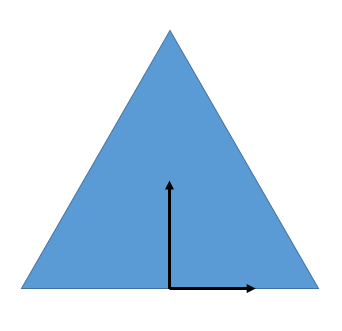
\includegraphics[scale=0.5]{./im/tri}
\end{wrapfigure}
\textbf{Método 1: Integral Doble }\\

Tome el marco de referencia como se muestra en la figura. Debido a la simetría del triangulo intuimos que en $x$ tenemos $x_{\text{cm}} = 0$ (lo demostraremos pero es bueno tener la intuición del resultado que esperamos). La región de integración está definida por las siguientes ecuaciones:


\begin{align*}
  -\frac{a}{2} \leq &x \leq \frac{a}{2}\\
 0 \leq &y \leq \left(\frac{a}{2} - |x|\right) \tan 60^{\circ}
\end{align*}

La expresión para calcular $y_{\text{cm}}$ es:


\begin{equation*}
\label{3} y_{\text{cm}} = \frac{1}{A} \int_{-a/2}^{a/2} \int_{0}^{ \left(\frac{a}{2} - |x|\right) \tan 60^{\circ}}   y\; dy dx
\end{equation*}

Se desarrolla la integral doble
\begin{equation*}
\label{4}  \int_{-a/2}^{a/2} \int_{0}^{ \left(\frac{a}{2} - |x|\right) \tan 60^{\circ}}   y\; dy dx = \frac{1}{2} \int_{-a/2}^{a/2} \left(\frac{a}{2} - |x|\right)^2 (\tan 60^{\circ})^2 dx = \frac{3}{2} \int_{-a/2}^{a/2} \left(\frac{a}{2} - |x|\right)^2  dx
\end{equation*}


Donde se usó $(\tan 60^{\circ})^2 = 3$. Se observa que el integrando es una función par por lo que se tiene:



\begin{equation*}
 \frac{3}{2} \int_{-a/2}^{a/2} \left(\frac{a}{2} - |x|\right)^2  dx = 3 \int_{0}^{a/2} \left(\frac{a}{2} - |x|\right)^2  dx =  3 \int_{0}^{a/2} \left(\frac{a}{2} - x\right)^2  dx
\end{equation*}

Usando el cambio de variable $u = \frac{a}{2} - x$ se obtiene:


\begin{equation*}
3 \int_{0}^{a/2} \left(\frac{a}{2} - x\right)^2  dx =  3 \int_{0}^{a/2} u^2 du = \frac{a^3}{8}
\end{equation*}

Por lo que finalmente se obtiene el centro de masa dividiendo por el área que es $A = \frac{\sqrt{3}}{4}a^2$:


\begin{equation*}
 y_{\text{cm}} = \frac{a}{2 \sqrt{3}}
\end{equation*}

Para la posición en $x$ del centro de masa (ya la sabemos pero verificamos el resultado):



\begin{equation*}
x_{\text{cm}} = \frac{1}{A} \int_{-a/2}^{a/2} \int_{0}^{ \left(\frac{a}{2} - |x|\right) \tan 60^{\circ}}   x\; dy dx = \frac{1}{A} \int_{-a/2}^{a/2}   \left(\frac{a}{2} - |x|\right)  x \tan 60^{\circ}\;  dx = 0
\end{equation*}

Donde se usó que la ultima integral tiene integrando impar. El centro de masa es:

\begin{equation}
\vec{\boldsymbol{r}}_{\text{cm}} =  \frac{a}{2 \sqrt{3}} \hat{\boldsymbol{\jmath}}
\end{equation}

\textbf{Método 2: Una sola Integral}\\


El problema se puede pensar como sumar rectángulos de ancho infinitesimal. El área de cada rectángulo es $dA = 2x' dy$, donde $x'$ es dado por $x'= a/2 - x$ y $x' \tan 60^{\circ} = y$. Es decir $x'$ es una distancia sobre una cara del triangulo equilátero, medida desde un vértice. $x$ es la distancia del centro de esa cara del triangulo al punto $x'$. Entonces $2x$ es el largo de nuestros rectángulos a integrar. La altura corre desde $0$ hasta la altura del triangulo, $\sqrt{3}a/4$. Por lo que la doble integral se reduce a la siguiente simple integral:  


\begin{equation*}
 y_{\text{cm}} = \frac{1}{A} \int_{0}^{\frac{\sqrt{3}}{2}a}  \left( a - \frac{2 y}{\tan 60^{\circ}} \right) y \; dy = \frac{a}{2\sqrt{3}}
\end{equation*}

\pagebreak
\section{Momentos de inercia}

\textbf{Partículas puntuales:}

El momento de inercia con respecto a un eje de rotación para un sistema discreto de $N$ partículas puntuales  está dado por:
\begin{equation}
I = \sum_{k=1}^{N} m_k r_k^2 = m_1 r_1^2 + \dots + m_N r_N^2
\end{equation}

Donde $ r_k$ es la distancia de la k-ésima partícula al eje y $m_k$ su masa. 

%\begin{wrapfigure}{r}{6.0cm}
%	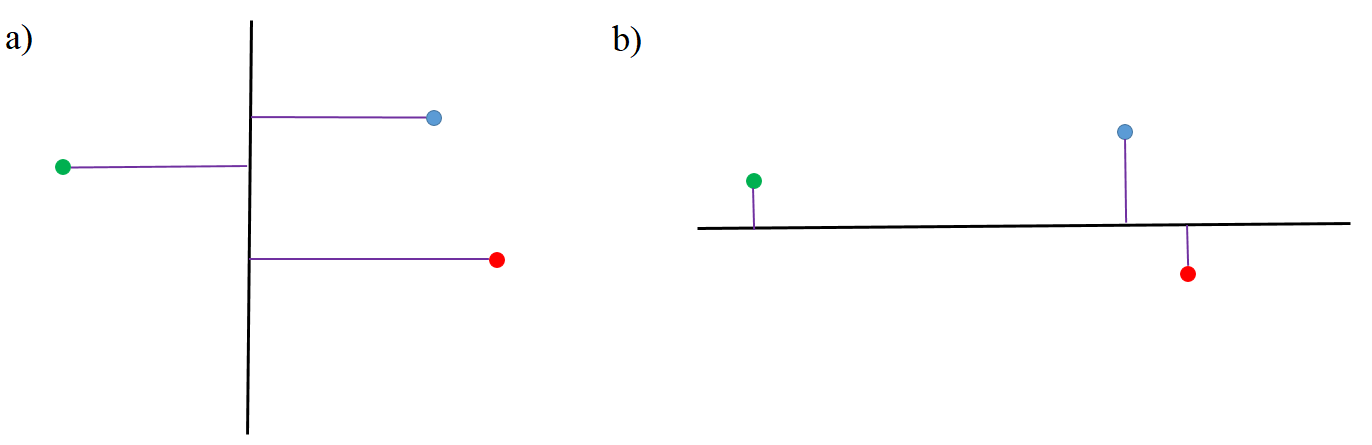
\includegraphics[scale=0.5]{./im/rot1}
%	\caption{Eje negro y las distancias en morado de las partículas al eje.}
%\end{wrapfigure}

\begin{figure}[H]
	\centering
	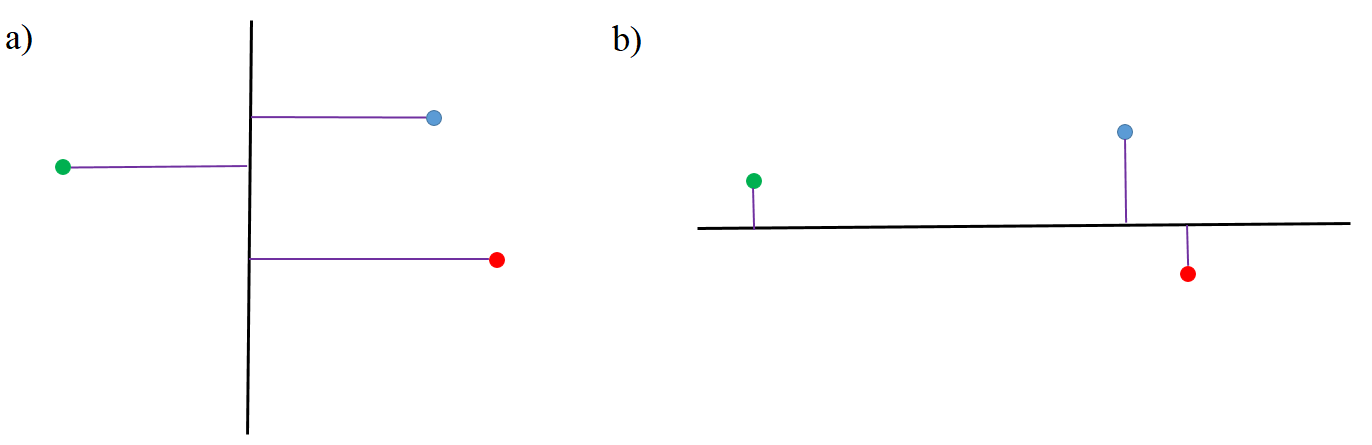
\includegraphics[width=\linewidth]{./im/rot1}
		\caption{Eje negro y las distancias en morado de las partículas al eje.}
\end{figure}

\vspace{1cm}







\textbf{Distribución continua:}


\vbox{\begin{wrapfigure}{r}{6.0cm}
	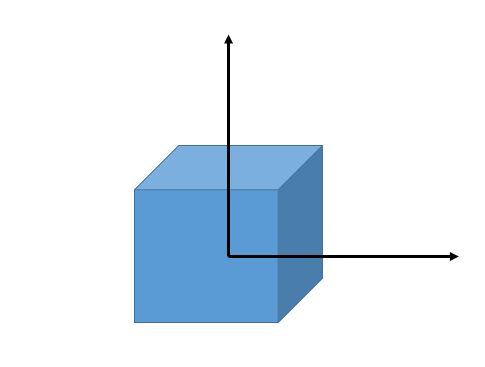
\includegraphics[scale=0.5]{./im/3d}
\end{wrapfigure}
El momento de inercia con respecto a un eje de rotación de un objeto con distribución de masa continua viene dado por la siguiente integral:

\begin{equation}
 I=  \int r^2 dm
\end{equation}}
\vspace{1cm}

Existen tres casos a considerar: objetos de 1, 2 y 3 dimensiones. Para cada una respectivamente existe una densidad asociada:

\begin{subequations}
	\begin{align}
	\lambda &= \frac{d m}{dx} \\
	\sigma &= \frac{d m}{dA} \\
	\rho &= \frac{d m}{dV} 
	\end{align}
\end{subequations}

Donde $\lambda$ es la densidad lineal, $\sigma$ la densidad superficial y $\rho$ la densidad (se omite decir densidad volumétrica, se le dice solo densidad usualmente). Con ellas se pueden obtener las siguientes expresiones para el centro de masa de distribuciones continuas:

\begin{subequations}
	\begin{align}
	I &=  \int r^2 \lambda \;dx  \\
	I &=  \int r^2 \sigma \;dA \\
	I &=  \int r^2 \rho\; dV 
	\end{align}
\end{subequations}


\subsection{Ejemplo 1: Anillo con densidad uniforme}


\begin{wrapfigure}{r}{5.0cm}
	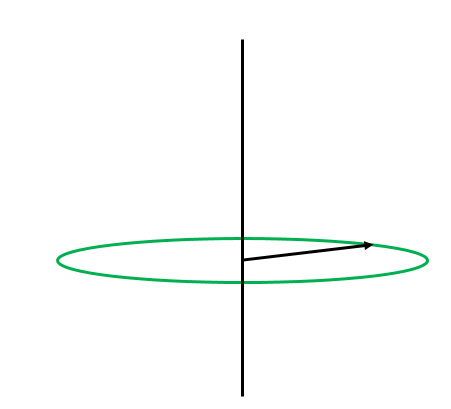
\includegraphics[scale=0.5]{./im/anillo1}
\end{wrapfigure}
Para calcular el momento de inercia de un anillo con respecto a un eje que pasa por el centro del anillo, perpendicular al plano donde este se encuentra, se debe hacer la siguiente integral:

$$ I = \int r^2 dm$$

El elemento de masa lo podemos expresar en términos del "volumen"(entre comillas ya que como el anillo es una figura de 1D, se considera su longitud y no volumen):

$$ dm = \lambda dr $$

Donde $\lambda$ es la densidad lineal dada por:

\begin{wrapfigure}{r}{4.0cm}
	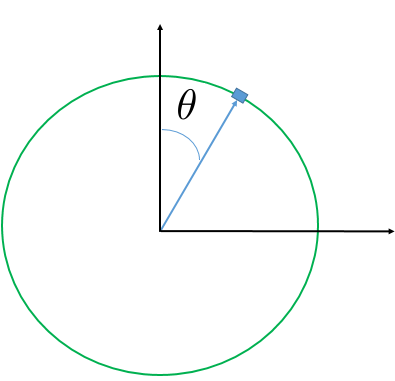
\includegraphics[scale=0.5]{./im/anillo2}
\end{wrapfigure}
$$ \lambda = \frac{M}{2 \pi R } $$

Y $dr$ es la posición del segmento infinitesimal del anillo que se está integrando. Como la posición de los segmentos siempre está a una distancia fija, esta posición se puede escribir en términos de un ángulo como:

$$ dr = R d\theta$$

Para recorrer todo el anillo, se debe dar una vuelta entera. Es decir $\theta$ va desde 0 hasta $2\pi$. Esto define los limites de la integral. Además se nota que la distancia desde el eje de rotación hasta cualquier parte del anillo siempre es $r=R$, por lo que se tiene:


$$ I = \int^{2\pi}_{0} \lambda  R^2 R d\theta$$

Como $\lambda$ y $R$ son constantes salen de la integral y se tiene:

$$ I = R^3 \lambda \int_{0}^{2\pi} d\theta = R^3 \lambda 2\pi = m R^2 $$


\subsection{Ejemplo 2: Disco de densidad uniforme}


\begin{wrapfigure}{r}{4.0cm}
	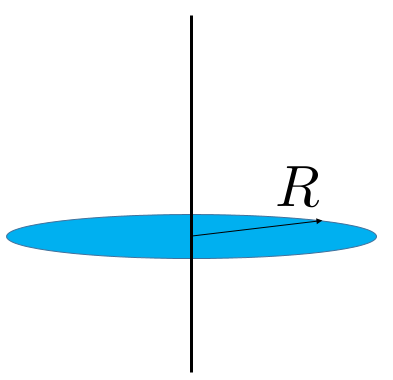
\includegraphics[scale=0.5]{./im/disc1}
\end{wrapfigure}

Se va a calcular el momento de inercia de un disco de masa $M$ distribuida uniforme. Este momento de inercia sera con respecto al eje que atraviesa el disco por el centro de masa (el centro) y perpendicular al plano del disco.


Para calcular el momento de inercia del disco vamos a dividir el disco en anillos y sumar la contribución de cada anillo. Estos anillos tiene un grosor infinitesimal $dr$. 
\vspace{2cm}
\begin{figure}[H]
	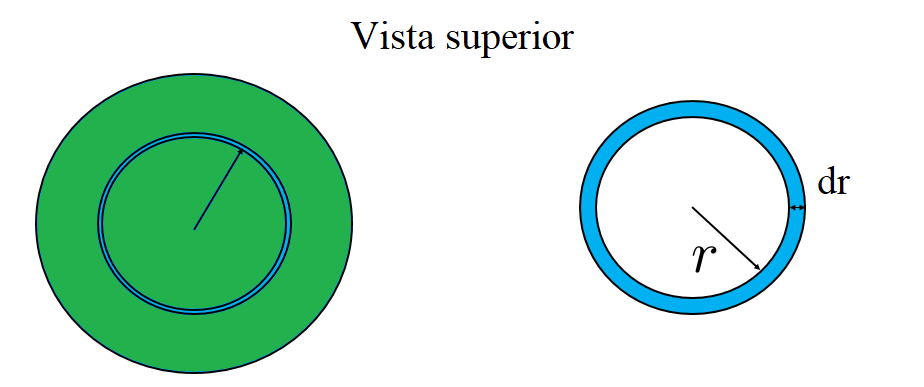
\includegraphics[width=\linewidth]{./im/disc2}
\end{figure}
\vspace{0.5cm}
Ya vimos que el momento de inercia de un anillo es:

$$ dI =  r^2 dm_a $$

Donde $dm_a$ es la masa de cada anillo que vamos a sumar y $r$ el radio de cada anillo. La integral se encarga de sumar cada anillo con grosor infinitesimal. Por lo tanto el momento de inercia esta dado por:

$$ I = \int d I  = \int r^2 dm_a $$

Para integrar cambiamos $dm_a$ usando la siguiente relación:

$$ dm_a = \sigma dA$$

Donde $dA$ es el área de cada anillo infinitesimal. Vemos que el área de cada anillo esta dado por la longitud del anillo por el grosor del anillo, es decir:

$$ dA = L dx = 2 \pi r d r$$

Juntando estos resultados el momento de inercia está dado por la siguiente expresión:
 
$$ I = \int \sigma r^2 2 \pi r dx$$

Recordando que la integral suma sobre todos los anillos, tenemos que variar $r$ desde el origen hasta el extremo del disco. Es decir que $r$ debe ir desde $0$ hasta $R$. Estos son entonces los limites de la integral:

$$ I =  \int_{0}^{R} \sigma 2\pi   r^3 dr$$

Como $\sigma$ y $2\pi$ son constantes, salen de la integral y se tiene:

$$ I =  2\pi\sigma \int_{0}^{R}    r^3 dr$$

Esta integral es:

$$ I =  2\pi\sigma \left( \frac{1}{4} R^4\right)$$

La densidad superficial $\sigma$ es:

$$ \sigma = \frac{m}{A} = \frac{m}{\pi R^2} $$

Finalmente, se obtiene el momento de inercia del disco:

$$ I = \frac{1}{2} m R^2$$

\subsection{Ejemplo 3: Cilindro de densidad uniforme}

Se va a calcular el momento de inercia de un cilindro de masa $M$ distribuida uniforme. Este momento de inercia se calcula con respecto a un eje que atraviesa el cilindro por el centro de masa (el centro) y perpendicular a las caras circulares del cilindro.
\vspace{1cm}

\begin{figure}[h]
	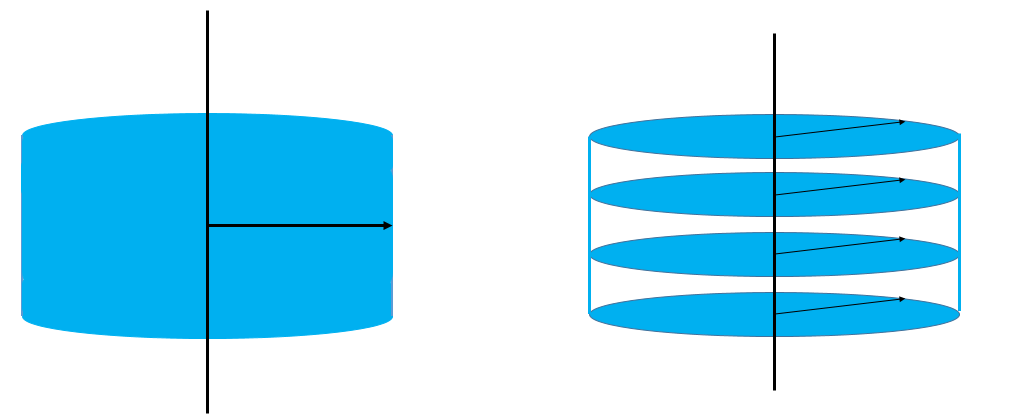
\includegraphics[width=\linewidth]{./im/cilindro1}
	
\end{figure}

\vspace{0.5cm}

Para calcular el momento de inercia del disco vamos a dividir el cilindro en discos y sumar la contribución de cada disco. Estos discos tienen un grosor infinitesimal $dy$. Ya vimos que el momento de inercia de un disco es:

$$ dI = \frac{1}{2} r^2 dm_d $$

Donde $dm_d$ es la masa de cada disco que vamos a sumar y $r$ el radio de cada disco. Como es un cilindro todos los discos tienen el mismo radio $R$. La integral se encarga de sumar cada disco con grosor infinitesimal. Por lo tanto el momento de inercia esta dado por:

$$ I = \int d I  = \frac{1}{2} \int R^2 dm_a $$

Como $R$ es una constante sale de la integral y se tiene:

$$ I = \frac{1}{2} R^2 \int dm_a$$

La integral $\int dm_a$ es la suma de la masa de todos los anillos, la cual es la masa total del cilindro $M$. Por lo tanto el momento de inercia es:

$$ I = \frac{1}{2} M R^2$$

Es el mismo que el del disco, solo que con la masa del cilindro. 

\subsection{Ejemplo 4: Bola de densidad uniforme}

Se va a calcular el momento de inercia de una bola de densidad uniforme con respecto a un eje que pasa por el centro de masa (el centro) de la bola.

\vspace{0.4cm}

\begin{figure}[H]
	\centering
	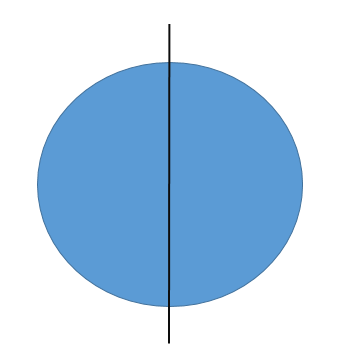
\includegraphics[width=0.5\linewidth]{./im/bola1}
	\caption{Bola y eje de rotación}
\end{figure}

\vspace{0.5cm}

Para calcular el momento de inercia de una bola vamos a dividir la bola en cilindros y sumar la contribución de cada cilindro. Estos cilindros tiene un grosor infinitesimal $dy$. 

\vspace{0.5cm}

\begin{figure}[H]
	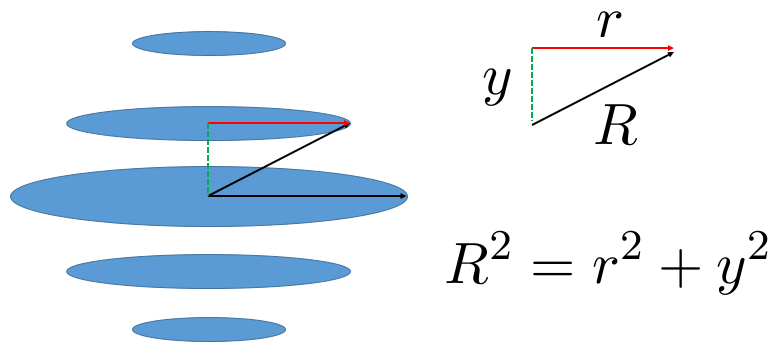
\includegraphics[width=1\linewidth]{./im/bola}
	\caption{Descomposición de bola en discos (cilindros de grosor infinitesimal).}
\end{figure}
\vspace{0.5cm}
Ya vimos que el momento de inercia de un cilindro es:
$$ dI = \frac{1}{2} r^2 dm_c $$

Donde $dm_c$ es la masa de cada cilindro que vamos a sumar y $r$ el radio de cada cilindro. La integral se encarga de sumar cada cilindro infinitesimal. Por lo tanto el momento de inercia esta dado por:

$$ I = \int d I  = \frac{1}{2}\int r^2 dm_c $$

Para integrar cambiamos $dm_c$ usando la siguiente relación:

$$ dm_c = \rho dV$$

Donde $dV$ es el volumen de cada cilindro infinitesimal. Vemos que el volumen de cada cilindro esta dado por el área del disco por el grosor cilindro, es decir:

$$ dV = A dy = \pi r^2 d y$$

Juntando estos resultados el momento de inercia está dado por la siguiente expresión:
 
$$ I = \frac{1}{2} \int \rho r^2 \pi r^2 dy$$

Ahora, para poder integrar esta expresión, tenemos que encontrar como depende el radio de los cilindros en función de la altura $y$. Usando el teorema de Pitágoras tenemos que:

$$ r^2 = R^2 - y^2$$

Por lo tanto el momento de inercia está dado por:

$$ I = \frac{1}{2} \int \rho \pi   (R^2-y^2)^2 dy$$

Recordando que la integral suma sobre todos los cilindros, tenemos que variar $y$ desde la parte inferior de la bola hasta la superior. Es decir que $y$ debe ir desde $-R$ hasta $R$. Estos son entonces los limites de la integral:

$$ I = \frac{1}{2} \int_{-R}^{R} \rho \pi   (R^2-y^2)^2 dy$$

Ahora lo único que falta es calcular la integral. Primero, note que la densidad y el número $\pi$ son constantes (no dependen de $y$), por lo que salen de la integral:

$$ I = \frac{1}{2} \rho \pi \int_{-R}^{R}    (R^2-y^2)^2 dy$$

Se expande la expresión $(R^2-y^2)^2$:

$$ (R^2-y^2)^2 = R^4 -2 R^2 y^2 + y^4$$

Ahora se reemplaza el resultado anterior en la integral:

$$ I = \frac{1}{2} \rho \pi \int_{-R}^{R}  R^4 -2 R^2 y^2 + y^4   dy$$

La integral es distributiva:
$$ I = \frac{1}{2} \rho \pi \left(  R^4\int_{-R}^{R} dy -2 R^2 \int_{-R}^{R} y^2 dy + \int_{-R}^{R}y^4   dy\right)$$

Las tres integrales anteriores son de monomios. Para un monomio de grado $n$ se conoce su integral:

$$ \int_{a}^{b} x^{n} dx = \left.\frac{x^{n+1}}{n+1}\right|_{a}^{b} = \frac{b^{n+1}}{n+1} - \frac{a^{n+1}}{n+1}$$

Juntando los resultados anteriores se obtiene el momento de inercia:

\begin{align*}
I &= \frac{1}{2} \rho \pi \left(  R^4(R-(-R))  -2 R^2 \left( \frac{R^3}{3}-\frac{(-R)^3}{3}\right)  + \left( \frac{R^5}{5}-\frac{(-R)^5}{5}\right)\right) \\
I  &=\frac{1}{2} \rho \pi \left(  2R^5 -2 R^5 \frac{2}{3}  + R^5 \frac{2}{5}\right)\\
I & = \frac{1}{2} \rho \pi R^5 \frac{16}{15}\\
I & = \frac{8}{15} \rho \pi R^5
\end{align*} 

El momento de inercia se puede escribir en terminos de la masa y el radio de la bola utilizando la expresión para su densidad:

$$ \rho = \frac{M}{V} = \frac{M}{\frac{4}{3} \pi R^3}$$

Finalmente, se obtiene el momento de inercia de una bola:

$$ I= \frac{8}{15} \frac{M}{\frac{4}{3} \pi R^3} \pi R^5 =  \frac{2}{5} M R^2$$

 

\section{Teorema de ejes paralelos}

El teorema de ejes paralelos da un formula para calcular el momento de inercia de un sistema con respecto a un eje de rotación que este paralelo a otro eje de rotación que pase por el centro de masa del objeto. Si $I_{cm}$ es el momento de inercia con respecto al eje que pasa por el centro de masa, y $a$ es la distancia entre dichos ejes se tiene que el momento de inercia del eje paralelo viene dado por:

\begin{equation}
 I_{a} = I_{cm} + M a^2
\end{equation}

\subsection{Ejemplo 1: Barra con eje en un extremo}

\begin{wrapfigure}{r}{7.0cm}
	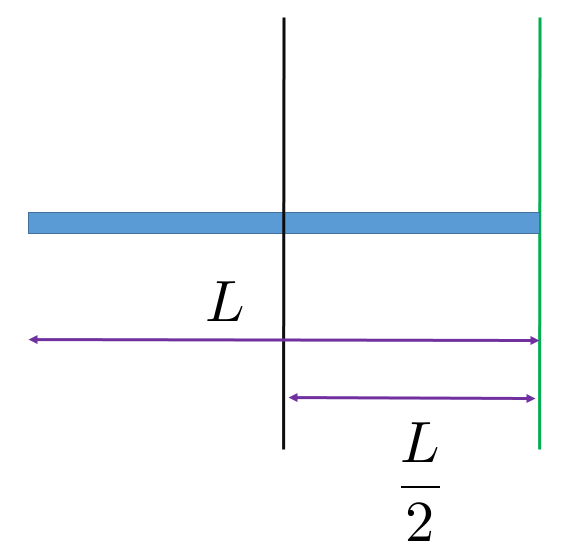
\includegraphics[scale=0.5]{./im/paralelobarra}
\end{wrapfigure}

El eje de la barra se encuentra a una distancia $L/2$ de un eje que es paralelo y pasa por el centro de masa. Por lo que por el teorema de ejes paralelos se tiene que el momento de inercia esta dado por la siguiente expresión:

$$ I = I_{cm} + m \left(\frac{L}{2}\right)^2$$

El momento con respecto al eje que pasa por el centro de masa es $I_{cm} =\frac{1}{12} m L^2$. 

$$ I = \frac{1}{3} m L^2$$

\vspace{1cm}

\subsection{Ejemplo 2: Bola con eje en un extremo}

\begin{wrapfigure}{r}{6.0cm}
	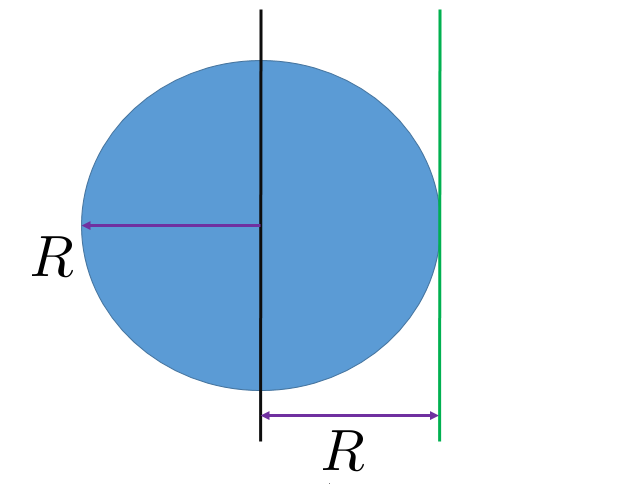
\includegraphics[scale=0.5]{./im/paralelobola}
\end{wrapfigure}

El eje de la bola se encuentra a una distancia $R$ de un eje que es paralelo y pasa por el centro de masa. Por lo que por el teorema de ejes paralelos se tiene que el momento de inercia esta dado por la siguiente expresión:

$$ I = I_{cm} + m R^2$$

El momento con respecto al eje que pasa por el centro de masa es $I_{cm} =\frac{2}{5} m R^2$. Entonces el momento de inercia es:

$$ I =\frac{2}{5} m R^2 + m R^2 = \frac{7}{5} m R^2$$

\pagebreak

\subsection{Ejemplo 3: 5 Discos}

En este ejemplo se tiene 5 discos de masa $m$ (cada uno) distribuida uniforme y todos con el mismo radio. Se quiere encontrar el momento de inercia con respecto a un eje que atraviesa el disco central por justo en el centro. Para hacerlo sumamos el momento de inercia de los 5 discos con respecto a dicho eje:

\begin{wrapfigure}{r}{6.0cm}
	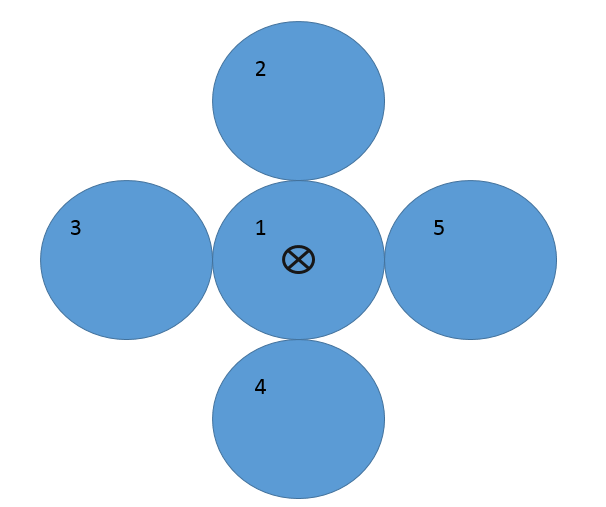
\includegraphics[scale=0.5]{./im/numerados}
\end{wrapfigure}

$$ I = I_1 + I_2 + I_3 + I_4 + I_5$$

Donde se $I_k$ es el momento de inercia del k-ésimo disco (en el dibujo se enumeran). El momento de inercia del disco 1 es respecto a un eje que atraviesa su centro de masa: $I_1 = 1/2 m R^2$. Para el disco 2 el eje es paralelo a su centro de masa a una distancia $2R$. Por lo que podemos usar el teorema de ejes paralelos:

$$ I_2 = I_{cm}  + m(2R)^2 = \frac{1}{2} mR^2 + 4 mR^2 = \frac{9}{2} m R^2$$

Para el disco 3,4 y 5 se tiene lo mismo, por lo que:

\begin{align*}
I &= I_1 + 4 I_2 = \frac{1}{2} mR^2 + 4 \left(\frac{9}{2} m R^2\right) = \frac{37}{2} m R^2 
\end{align*}


\end{document}
